\chapter[$\mathcal{H}_\infty$ approch for reference model in DDDC]{Model selection for Direct data-driven control through $\mathcal{H}_\infty$ techniques}
Here the objective is to describe a systematic approach by which a \textit{Reference Model} $M(q^{-1})$, that can be used in the framework of DDDC, can be obtained given suitable \textit{quantitative performance requirements}. In the literature (see \citeauthor*{campestrini2016unbiased} \cite{campestrini2016unbiased} and \citeauthor*{da2018choice} \cite{da2018choice}) several valid guidelines are provided about this topic, however they do not explicitly take into account for performance requirements.

\begin{figure}[h]
    \centering
    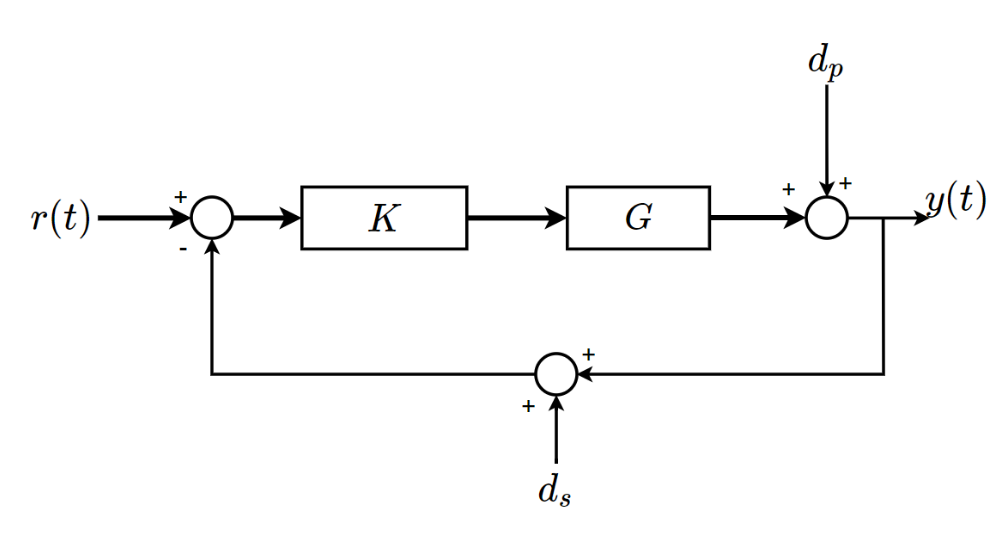
\includegraphics[scale=0.3]{img/RefMod_1.png}
    \caption{General FCS with disturbance and reference}
    \label{fig: gen_FCS}
\end{figure}

In general, we want to find a reference model $M$ that is able to take into account both tracking and disturbance/noise rejection. \\
\textit{Standard approaches} which address the problem of designing a reference model, are aimed to impose a certain behaviour to the complementary sensitivity function $T(q^{-1})$ of the system in \Cref{fig: gen_FCS}. For example:
\begin{itemize}
    \item \textsf{Prototype I Order System} the step response can be obtain, in the frequency domain, as 
    \begin{equation}\label{eq:prot_first}
        M(s)=\frac{1}{1+\frac{s}{p}}
    \end{equation}
    the time constant $1/p$ is the only degree of freedom which is used in order to obtain faster/slower rise time, in this case no oscillations and overshoot occur.
     \item \textsf{Prototype II Order System} We aim at building a reference model $M$ as follows: 
     \begin{equation}\label{eq:prot_second}
        M(s)=\frac{\omega_n^2}{s^2+2\zeta\omega_n{s}+\omega_n^2}
     \end{equation}
     here according to the parameter $\zeta$ different damping properties can be obtained (oscillations in the step response), the time constant $1/{\zeta\omega_n}$ is tuned in order to obtain certain convergence properties.
\end{itemize}

\noindent
It seems that all the needed performances can be achieved by properly tuning the parameters of such prototype models. However, it is remarkable that the input/output behaviour of the feedback control system in \Cref{fig: gen_FCS} is given by: 
\begin{equation}
    y=Tr+S{d_p}+T{d_s}
\end{equation}
Even if the function $S(q^{-1})=1-T(q^{-1})$ directly depends on the complementary sensitivity function whose shape can be decided using \Cref{eq:prot_first} and \Cref{eq:prot_second}, it is not said at all that it enjoys good attenuation properties with respect to the disturbance $d_p(t)$ acting on the plant! \\
The \textbf{proposed approach} is to design $M(q^{-1})$ by solving a fictitious control design problem accounting for all the quantitative performance requirements involved in the considered control problem.

\section{Model reference design: the $\mathcal{H}_\infty$ approach}
Here we consider the problem of designing $M(q^{-1})$ by solving a fictitious control problem in the framework of the $\mathcal{H}_\infty$ optimization (see \citeauthor*{cerone2020h} \cite{cerone2020h}). Common classes of \textbf{quantitative performance requirements} are: 
\begin{itemize}
    \itemsep-0.3em
    \item steady-state response to polynomial reference inputs
    \item steady-state response to polynomial disturbance $d_p$ 
    \item steady-state response to measurement disturbance $d_s$
    \item transient step response requirements in term of: rise time $t_r$, settling time $t_{s,\alpha\%}$ and overshoot $\hat{s}$.    
\end{itemize}
It is well known that in the context of $\mathcal{H}_\infty$ control, performance requirements can be translated into frequency domain constraints on a \textbf{weighted} $\mathcal{H}_\infty$-norm on the sensitivity function ($S$) and complementary sensitivity function ($T$):
\begin{align}
    \Vert W_T(j\omega) T(j\omega) \Vert_\infty \le 1\\
    \Vert W_S(j\omega) S(j\omega) \Vert_\infty \le 1
\end{align}

\subsection{Case 1: stable and minimum phase plant}
When the unknown plant is stable and minimum phase the problem of finding a reference model $M(s)$ is given by:
\begin{equation}
    M(s)=\tilde{T}(s)=\frac{\tilde{K}(s)\tilde{G}(s)}{1+\tilde{K}(s)\tilde{G}(s)}
\end{equation}
where $\tilde{K}(s)$ is the controller obtained by solving the optimization problem:
\begin{equation}
    \tilde{K}(s)=\arg\min_{\tilde{K}\in \tilde{K}(s)^{stab}} {\Vert T_{wz}(s)} \Vert_\infty
\end{equation}
where $T_{wz}$ is the closed  loop transfer function between the input $w$ and the output $z$, and $W_S$ and $W_T$ are rational transfer function designed taking into account frequency domain constraints imposed by performance requirements, that is
\begin{equation}
    T_{wz}(s)=\begin{bmatrix}
        W_T \tilde{T}\\
        W_S \tilde{S}
    \end{bmatrix}
\end{equation}
the block-diagram of the general control configuration we are referring to is the one depicted in \Cref{fig:gen_plant} which is the generalized plant for \textit{nominal performance requirements}.

\begin{figure}[h]
    \centering
    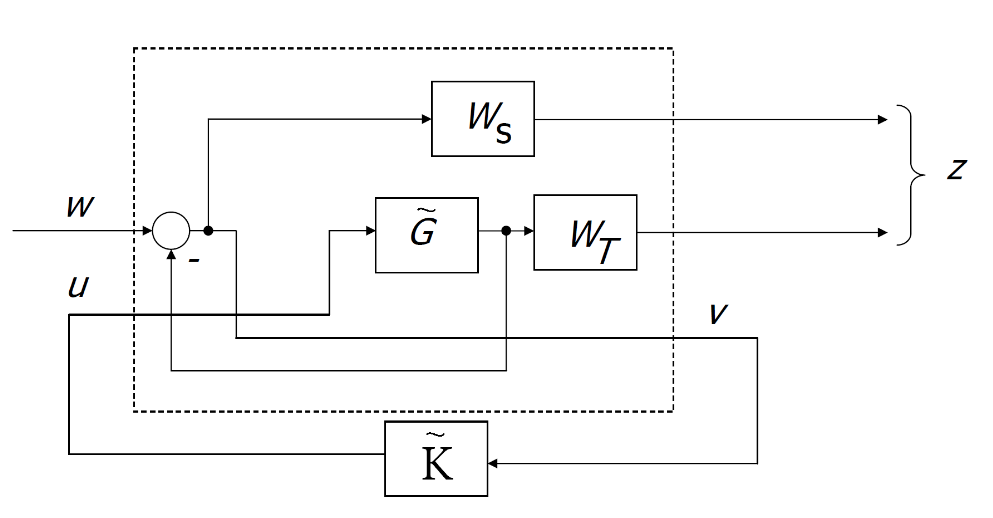
\includegraphics[scale=0.35]{img/gen_plant.png}
    \caption{Generalized plant for nominal performances}
    \label{fig:gen_plant}
\end{figure}
\begin{remark}
    The controller $\tilde{K}$ is instrumental to the computation of $\tilde{T}$ and then the reference model $M$. In other words the controller $\tilde{K}$ does not solve the problem for the actual plant which is unknown.
\end{remark}

\subsection{Case 2: stablle non-minimum phase systems}
\begin{definition}[\textbf{Non-minimum phase system}]
    
A non-minimum phase system is a dynamic system whose transfer function has one or more zeros in the right-half of the s-plane (for continuous-time systems) or outside the unit circle (for discrete-time systems). These zeros lead to certain undesirable characteristics, particularly in transient response and stability.
\end{definition}

Step-response of non-minimum phase exhibit \textit{undershoot}, in particular it is a behaviour of  the transient response of a system where the output initially moves in the direction opposite to the desired final value before eventually settling at the target.\\

In this case, the reference model can be designed using the $\mathcal{H}_\infty$ approach, but instead of selecting $\tilde{G}=1$ as fictitious plant, we include all the NMP zeros of the plant a number of poles equals or greater than the NMP ones. The additional poles are chosen in arbitrary way\footnote{
    It is well-known that stable poles do not induce any performance limitation in the feedback control system.
} under the condition that they are stable, moreover if the system type is greater or equal than one a suitable number of poles at the origin can be included in $\tilde{G}$.

\subsection{Last step: Discretization of $M(s)$}
Since in the DDDC based on the SM approach, we use a discrete-time description, the reference model is supposed to be discretized using a suitable sampling time $T_s$, obtaining then the reference model $M(q^{-1})$

\section{Simulation example and discussion}
In this example, we use the proposed approach to tune a controller for a SISO NMP plant. A numerical comparison with the standard approach is presented. Here we assume that the plant is a NMP system described by the following transfer function
\begin{equation}
    G(s)=\frac{(s+9.925)(s-1.818)}{(s+12.04)(s+2.231)}
\end{equation}
the disturbances are
\begin{equation}
    \begin{aligned}
        &d_p(t)=a_p\sin(\omega_p{t}), \ \vert a_p \vert \le 2\cdot{10^{-2}}, \ \omega_p \le 0.02 \text{rad \ s}^{-1}\\
        &d_s(t)=a_s\sin(\omega_s{t}), \ \vert a_s \vert \le {10^{-1}}, \ \omega_s \le 40 \ \text{rad \ s}^{-1}\\
    \end{aligned}
\end{equation}

The \Cref{tab:performance} reports the time domain specifications and the performances achieved with the contrrolled systems obtained with the two approaches (SMRC) and ($\mathcal{H}_\infty$RMC).

\begin{table}[h!]
\centering
\begin{tabular}{|>{\raggedright\arraybackslash}m{5cm}|>{\centering\arraybackslash}m{3cm}|>{\centering\arraybackslash}m{3cm}|>{\centering\arraybackslash}m{3cm}|}
\hline
\textbf{Performance Specifications} & \textbf{Upper Bound Value} & \textbf{SRMC} & \textbf{$H_\infty$RMC} \\ \hline
Steady-state output error when the reference is a ramp & 0.5 & \textbf{0.7} & 0.495 \\ \hline
Steady-state output error in the presence of $d_p$ & $6 \cdot 10^{-4}$ & $2.84 \cdot 10^{-4}$ & $2.22 \cdot 10^{-4}$ \\ \hline
Steady-state output error in the presence of $d_s$ & $8 \cdot 10^{-3}$ & \textbf{0.0196} & $6.83 \cdot 10^{-3}$ \\ \hline
Step response overshoot & 11\% & \textbf{11.5\%} & 9.77\% \\ \hline
Rise time & 2 (s) & 0.939 (s) & 0.988 (s) \\ \hline
Settling time & 8 (s) & 6.36 (s) & 7.33 (s) \\ \hline
\end{tabular}
\caption{Performance Comparison}
\label{tab:performance}
\end{table}

It is remarkable that even if the two step-responses are quite similar, the controlled system designed by using the standard approach does not fulfill all the requirements, on the contrary the proposed approach fulfills all of the performance requirements.